\documentclass{article}
\usepackage[utf8]{inputenc}

\title{Linear Algebra Applications to Cryptography}
\author{Emily Nomura}
\date{MATH 0520, Section S03, Spring 2018}

\usepackage{natbib}
\usepackage{graphicx}
\usepackage{amsmath}
\setcounter{MaxMatrixCols}{20}

\begin{document}
\maketitle

\section{Introduction}
Linear Algebra has many real-world applications, including to artificial intelligence, economics, video game graphics, and even basic geometry. One of the most interesting applications of linear algebra is cryptography, “the study of the techniques of writing and decoding message in code”\cite{ref1:1}. 

\section{Cryptography: What is it?}
 One may be more familiar with the term ``encryption" rather than cryptography. Encryption is defined as the transformation of data into some type of form that is unreadable to the human eye. Decryption is the opposite of encryption - the transformation of unreadable data into something that is readable. Some other common cryptography terms are ``plaintext" and ``ciphertext." Plaintext is the message that is being encrypted and ciphertext is the information that is revealed after the plaintext has been decrypted \cite{ref1:1}. The ``key" is the method used to decipher the message. In certain cases, encryption and decryption use the same key. However, in more complex cases, encryption and decryption may use different keys to move between the plaintext and ciphertext. Below is a set of equations for a simple cryptography process where $P$ is the plaintext, $C$ is the ciphertext, $E$ is the encryption method, $D$ is the decryption method, and $k$ is the key \cite{ref2:2}.

{\center $C = E_{k}(P)$\\
$P = D_{k}(C)$
\endcenter}

\section{Cryptography: Why do we need it?}
Personal financial information such as credit card numbers, paychecks, and bank statements are all stored online. In addition, sensitive information like electronic health records can often be accessed on the web through a health services patient portal. Cryptography is essential to ensuring the privacy of these types of information.\\

Kessler states that there are five main functions of cryptography \cite{ref2:2}:
\begin{enumerate}
    \item Confidentiality: ensuring that no one can read the message other than the intended receiver.
    \item Authentication: the process of proving one’s identity online.
    \item Integrity: a way of assuring that the receiver has received the message in its intended form.
    \item Non-repudiation: a mechanism to prove that the person sending the message actually sent that message.
    \item Key exchange: a method in which the key is sent between the sender and the receiver of the message in order to decrypt the encryped message.
\end{enumerate}
%In general, cryptography is associated with the development and creation of the “mathematical algorithms used to encrypt and decrypt messages,” while cryptoanalysis deals with breaking down encryptions and analyzing them \cite{ref2:2}.

\section{The Caesar Cipher}
One of the most basic examples of cryptography is the Caesar Cipher, also known as the shift cipher. The Caesar Cipher is solved using a substitution process where each letter in the plaintext is replaced with another letter. The replacement letter is determined by the shift key. For example, a shift key of $+3$ should shift each letter in the message up three units. Most Caesar Ciphers only use positive integers as the shift key. However, a shift key can also be negative, resulting in a shift down the alphabet. A shift key of $+3$ is also known as a ``left shift of 3,” illustrated in Figure 1.\\

\begin{figure}[h]
    \centering
    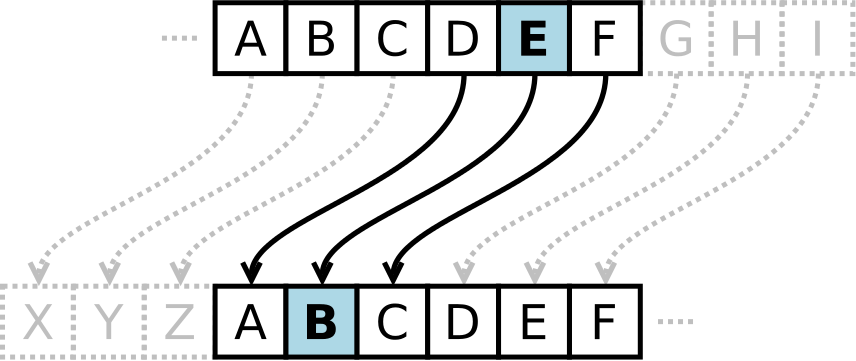
\includegraphics[scale=0.4]{caesar_cipher}
    \caption{Caesar Cipher key of $+3$}
    \label{fig:enter-label}
\end{figure}

\subsection{Mathematics}
The encryption of a Caesar Cipher can be expressed as an equation \cite{ref3:3}:

$$ E_{n}(x) = x + n  (\text{mod }26)$$\\
The decryption process can be expressed similarly.

$$ D_{n}(x) = x - n  (\text{mod }26)$$

\noindent
The Caesar Cipher is a simple and well-known form of encryption that is easy to understand. However, it is not a safe or reliable way to encrypt sensitive information. There are many more advanced forms of cryptography, some of which rely on linear algebraic operations.

\section{Linear Algebra Applications}
Many governments in this day and age are using more and more sophisticated and complicated methods of coding and decoding to try and keep information private. One of the best ways of performing encryptions is with a simple 3 by 3 matrix. The first matrix given is dubbed the “encoding matrix” while its inverse is called the “decoding matrix” \cite{ref4:4}.

\subsection{Example 1}
The following example can be found at the second reference source, and uses a 3 by 3 matrix to enrypt and then decrypt the message PREPARE TO NEGOTIATE.
{\center
Encoding matrix = 
$$
\begin{bmatrix}
-3 & -3 & -4 \\
0 & 0 & 1 \\
4 & 3 & 4 
\end{bmatrix}
$$
\endcenter}

\noindent
The message consists of three words; each letter of this message will correspond to a certain number. For the simplicity of this particular example, each letter will be associated with its corresponding position in the alphabet. For example, “A” will be assigned to the value “1,” “B” to “2,” and so on. For a space, which, in this case, will occur twice since there are three words and two spaces in between each word, will correspond to the number 27, one number after 26 which corresponds to the last letter of the alphabet, “Z.” The message, once translated into the corresponding numbers, becomes this sequence of numbers:

$$
16, 18, 5, 16, 1, 18, 5, 27, 20, 15, 27, 14, 5, 7, 15, 20, 9, 1, 20, 5
$$

\noindent
Since the encoding matrix is a 3 by 3 matrix, the message will then be broken up into a sequence of column vectors that are size 3. This will look as follows:

$$
\begin{bmatrix}
16\\
18\\
5
\end{bmatrix}
\begin{bmatrix}
16\\
1\\
18
\end{bmatrix}
\begin{bmatrix}
5\\
27\\
20
\end{bmatrix}
\begin{bmatrix}
15\\
27\\
14
\end{bmatrix}
\begin{bmatrix}
5\\
7\\
15
\end{bmatrix}
\begin{bmatrix}
20\\
9\\
1
\end{bmatrix}
\begin{bmatrix}
20\\
5\\
27
\end{bmatrix}
$$ \\

\noindent
As one might notice, the message contains 20 characters total including the spaces. There are 7 column vectors of size 3, meaning that there are actually 21 characters when put in this format. This is because each vector MUST be of size 3 since we will be multiplying them with the encoding matrix. Thus, a 27 must be added at the end of the message representing a space to keep all vectors of the same size. Next, the sequence of column vectors are put together into a 3 by 7 matrix, and multiplied with the encoding matrix. This computation step will look like this:

$$
\begin{bmatrix}
-3 & -3 & -4 \\
0 & 0 & 1 \\
4 & 3 & 4 
\end{bmatrix}
\quad
\begin{bmatrix}
16 & 16 & 5 & 15 & 5 & 20 & 20 \\
18 & 1 & 27 & 27 & 7 & 9 & 5 \\
5 & 18 & 20 & 14 & 15 & 1 & 27
\end{bmatrix}
$$
\\
\noindent
Since we are multiplying a 3 by 3 matrix with a 3 by 7 matrix, this matrix multiplication is possible since n = 3 in the first matrix and m = 3 in the second matrix. The resulting matrix will be a 3 by 7 matrix that looks like this:

{\center
Message matrix =
$$
\begin{bmatrix}
-122 & -123 & -176 & -182 & -96 & -91 & -183 \\
23 & 19 & 47 & 41 & 22 & 10 & 32 \\
138 & 139 & 181 & 197 & 101 & 111 & 203
\end{bmatrix}
$$
\endcenter}
\\
\noindent
The work done up until this point is done by the sender. The receiver will receive this 3 by 7 matrix and the encoding matrix. Then, they will proceed to decode this matrix. In order to decode this 3 by 7 matrix, the receiver must find the inverse of the encoding matrix to get the decoding matrix. As we learned in class, the inverse of a 3 by 3 matrix can be found easily by expanding the 3 by 3 matrix into a 3 by 6 matrix with the standard 3 by 3 matrix as the rightmost 3 columns. Row operations are used to get the standard 3 by 3 matrix on the left size, and the corresponding matrix on the right side is the inverse of the original matrix. For simplicity, the inverse of the matrix, also known as the decoding matrix, has already been computed.

{\center
Decoding matrix =
$$
\begin{bmatrix}
1 & 0 & 1 \\
4 & 4 & 3 \\
-4 & -3 & -3
\end{bmatrix}
$$
\endcenter}

\noindent
After the decoding matrix is computed, it is multiplied by the 3 by 7 matrix that the receiver received in order to get the final 3 by 7 matrix. This matrix is then expanded by the receiver going through each successive column vector (of size 3) and is translated to each corresponding letter of the alphabet. Below is the resulting matrix and the corresponding sequence of numbers which is the same as earlier depicted. This sequence of numbers exactly corresponds to the original message, PREPARE TO NEGOTIATE. The multiplication of the decoding matrix with the message is not shown. It will be shown in Example 2. \\
\\
{\center
$$
\begin{bmatrix}
16 & 16 & 5 & 15 & 5 & 20 & 20 \\
18 & 1 & 27 & 27 & 7 & 9 & 5 \\
5 & 18 & 20 & 14 & 15 & 1 & 27
\end{bmatrix} \\
16, 18, 5, 16, 1, 18, 5, 27, 20, 15, 27, 14, 5, 7, 15, 20, 9, 1, 20, 5
$$
\endcenter}

{\center
Message = PREPARE TO NEGOTIATE
\endcenter}

\subsection{Example 2}
\noindent
This original example follows the same format as Example 1. The receiver will receive both the encoding matrix and the message matrix. They will do the computation below which includes computing the inverse of the encoding matrix and multiplying it with the message matrix. The receiver will then translate each number to the corresponding letter in order to decode the message. \\

\noindent
Message = I LOVE MATH TO A CERTAIN EXTENT \\

\noindent
Sequence of numbers = 
$$
9, 27, 12, 5, 22, 5, 27, 13, 1, 20, 8, 27, 20, 15, 27, 1, 27, 3, 5, 18, 20, 1, 9, 14, 27, 5, 24, 20, 5, 14, 20
$$
{\center
Message = 
$$
\begin{bmatrix}
9\\
27\\
12
\end{bmatrix}
\begin{bmatrix}
15\\
22\\
5
\end{bmatrix}
\begin{bmatrix}
27\\
13\\
1
\end{bmatrix}
\begin{bmatrix}
20\\
8\\
27
\end{bmatrix}
\begin{bmatrix}
20\\
15\\
27
\end{bmatrix}
\begin{bmatrix}
1\\
27\\
3
\end{bmatrix}
\begin{bmatrix}
5\\
18\\
20
\end{bmatrix}
\begin{bmatrix}
1\\
9\\
14
\end{bmatrix}
\begin{bmatrix}
27\\
5\\
24
\end{bmatrix}
\begin{bmatrix}
20\\
5\\
14
\end{bmatrix}
\begin{bmatrix}
20\\
27\\
27
\end{bmatrix}
$$ \\

Encoding matrix = 
$$
\begin{bmatrix}
3 & 3 & -1\\
-2 & -2 & 1\\
-4 & -5 & 2
\end{bmatrix}
$$
\endcenter}

\noindent
Multiplying the encoding matrix and message composed of column vectors of size 3 to find the message matrix:
{\center
$$
\begin{bmatrix}
3 & 3 & -1 \\
-2 & -2 & 1 \\
-4 & -5 & 2
\end{bmatrix}
\quad
\begin{bmatrix}
9 & 15 & 27 & 20 & 20 & 1 & 5 & 1 & 27 & 20 & 20 \\
27 & 22 & 13 & 8 & 15 & 27 & 18 & 9 & 5 & 5 & 27\\
12 & 5 & 1 & 27 & 27 & 3 & 20 & 14 & 24 & 14 & 27
\end{bmatrix}
$$ \\
Message matrix =
$$
\begin{bmatrix}
96 & 106 & 115 & 57 & 78 & 81 & 49 & 16 & 72 & 61 & 114\\
-60 & -69 & -79 & -29 & -43 & -53 & -26 & -6 & -40 & -36 & -67 \\
-147 & -160 & -171 & -66 & -101 & -133 & -70 & -21 & -85 & -77 & -161
\end{bmatrix}
$$ \\
Decoding matrix =
$$
\begin{bmatrix}
1 & -1 & 1\\
0 & 2 & -1\\
2 & 3 & 0
\end{bmatrix}
$$
\endcenter}

\noindent
Multiplying the decoding matrix and message matrix to find the original message which can then be converted to the corresponding letters:
{\center
$$
\begin{bmatrix}
1 & -1 & 1\\
0 & 2 & -1\\
2 & 3 & 0
\end{bmatrix}
\quad
\begin{bmatrix}
96 & 106 & 115 & 57 & 78 & 81 & 49 & 16 & 72 & 61 & 114\\
-60 & -69 & -79 & -29 & -43 & -53 & -26 & -6 & -40 & -36 & -67 \\
-147 & -160 & -171 & -66 & -101 & -133 & -70 & -21 & -85 & -77 & -161
\end{bmatrix}
$$ \\

Final message =
$$
\begin{bmatrix}
9 & 15 & 27 & 20 & 20 & 1 & 5 & 1 & 27 & 20 & 20 \\
27 & 22 & 13 & 8 & 15 & 27 & 18 & 9 & 5 & 5 & 27\\
12 & 5 & 1 & 27 & 27 & 3 & 20 & 14 & 24 & 14 & 27
\end{bmatrix}
$$

Sequence of numbers =
$$
9, 27, 12, 5, 22, 5, 27, 13, 1, 20, 8, 27, 20, 15, 27, 1, 27, 3, 5, 18, 20, 1, 9, 14, 27, 5, 24, 20, 5, 14, 20
$$

Message = I LOVE MATH TO A CERTAIN EXTENT
\endcenter}

\section{Conclusion}
This relatively simple example of encryption through a 3 by 3 matrix is highly effective; at least much more effective than a Caesar Cipher. However, it is important to remember that although encryption is necessary for secure communications, it is not sufficient enough by itself. Many other steps are necessary for the utmost security. There are many levels to cryptography, ranging from simple (like the Caesar Cipher) to medium difficulty (like using matrix multiplication and inverses) to a variety of nearly unbreakable methods that top-notch governments and cryptographers use. As one of the most interesting applications of linear algebra, Cryptography is a complicated yet rewarding process that will be used and implemented well into the future. \\

\newpage
\bibliography{references}
\bibliographystyle{ieeetr}

\end{document}